\chapter{Preprocessing Patterns, Term-Templates, and Top-Level Forms}

This section describes Transformation/Analysis Passes that are applied to patterns and \texttt{define-language} forms. Most of these are based on \texttt{Visitor} classes described in Section \ref{section:visitors}.


\section{Pattern: Pattern-Variable Resolution}
\label{section:pv-resolve}

\subsection{Algorithm}

Immediately after parsing the PLTRedex specification, it is unknown whether certain elements of a pattern are built-in patterns, non-terminal symbols or just literals. These elements are represented with \UnresolvedSymbol instances and will have to be resolved in one of the following ways: \BuiltInPatternNoArg, \NonTerminalNoArg, or \LiteralPatternNoArg.

If this transformation is being applied to \texttt{define-language} form, all sub-patterns that resolve to \LiteralPatternNoArg \space need to be stored in set $V$ (initially empty) which is the set of all variables used by the given language. After applying the transformation, \texttt{define-language} $l$ form has to be annotated with $V$ - \MakeAnnotation{$l$}{"ReservedVariables"}{$V$}.

Given \LetDefineLanguage{$l$}, let $\mathit{Nt_{l}}$ be the set of all non-terminal symbols of the language. Given string $\mathit{sym}$, the prefix of $\mathit{sym}$ needs to be extracted. Let $\mathit{prefix_{sym}}$ be a string of characters up to the first occurrence of an underscore character in $\mathit{sym}$. There are several cases to consider.

\begin{itemize}
\item $\mathit{prefix_{sym}}$ does not exist; there are no underscore characters in $\mathit{sym}$. Let $\mathit{prefix_{sym}=sym}$.
\item $\mathit{prefix_{sym}}$ is empty; the first character of $\mathit{sym}$ is underscore. Raise an Exception because PLTRedex doesn't consider such symbols valid.
\item Otherwise, $\mathit{prefix_{sym}}$ is the prefix.
\end{itemize}

The resolution algorithm proceeds in the following manner. The pattern is traversed recursively. When coming across \UnresolvedSymbol \space node, extract $\mathit{prefix_{sym}}$. One of the following cases may happen.

\begin{itemize}
\item Prefix is \texttt{number}, return \BuiltInPattern[Number][$\mathit{sym}$][false].
\item Prefix is \texttt{integer}, return \BuiltInPattern[Integer][$\mathit{sym}$][false].
\item Prefix is \texttt{real}, return \BuiltInPattern[Real][$\mathit{sym}$][false].
\item Prefix is \texttt{natural}, return \BuiltInPattern[Natural][$\mathit{sym}$][false].
\item Prefix is \texttt{string}, return \BuiltInPattern[String][$\mathit{sym}$][false].
\item Prefix is \texttt{boolean}, return \BuiltInPattern[Boolean][$\mathit{sym}$][false].
\item Prefix is \texttt{variable-not-otherwise-mentioned}, \\ return \BuiltInPattern[Variable][$\mathit{sym}$][false]
\item Prefix is \texttt{hole}. Since PLTRedex doesn't allow underscores for \texttt{hole} patterns check if $\mathit{prefix(sym) \neq sym}$ and raise an Exception accordingly. \\ Return \BuiltInPattern[Hole][$\mathit{sym}$][false].
\item $\mathit{prefix_{sym} \in Nt_l}$, return \NonTerminal[$\mathit{prefix_{sym}}$][$\mathit{sym}$][false].
\item Finally, ensure that symbol does not contain underscores. PLTRedex only allows underscores after non-terminal symbols and built-in patterns. Abort compilation process if that is the case. Otherwise, $V=V\cup\{\mathit{sym}\}$ and return \LiteralPattern[Variable][$\mathit{sym}$][false]
\end{itemize}

\subsection{Example}

\begin{figure}[ht]
	\makebox[\textwidth][c] { 
		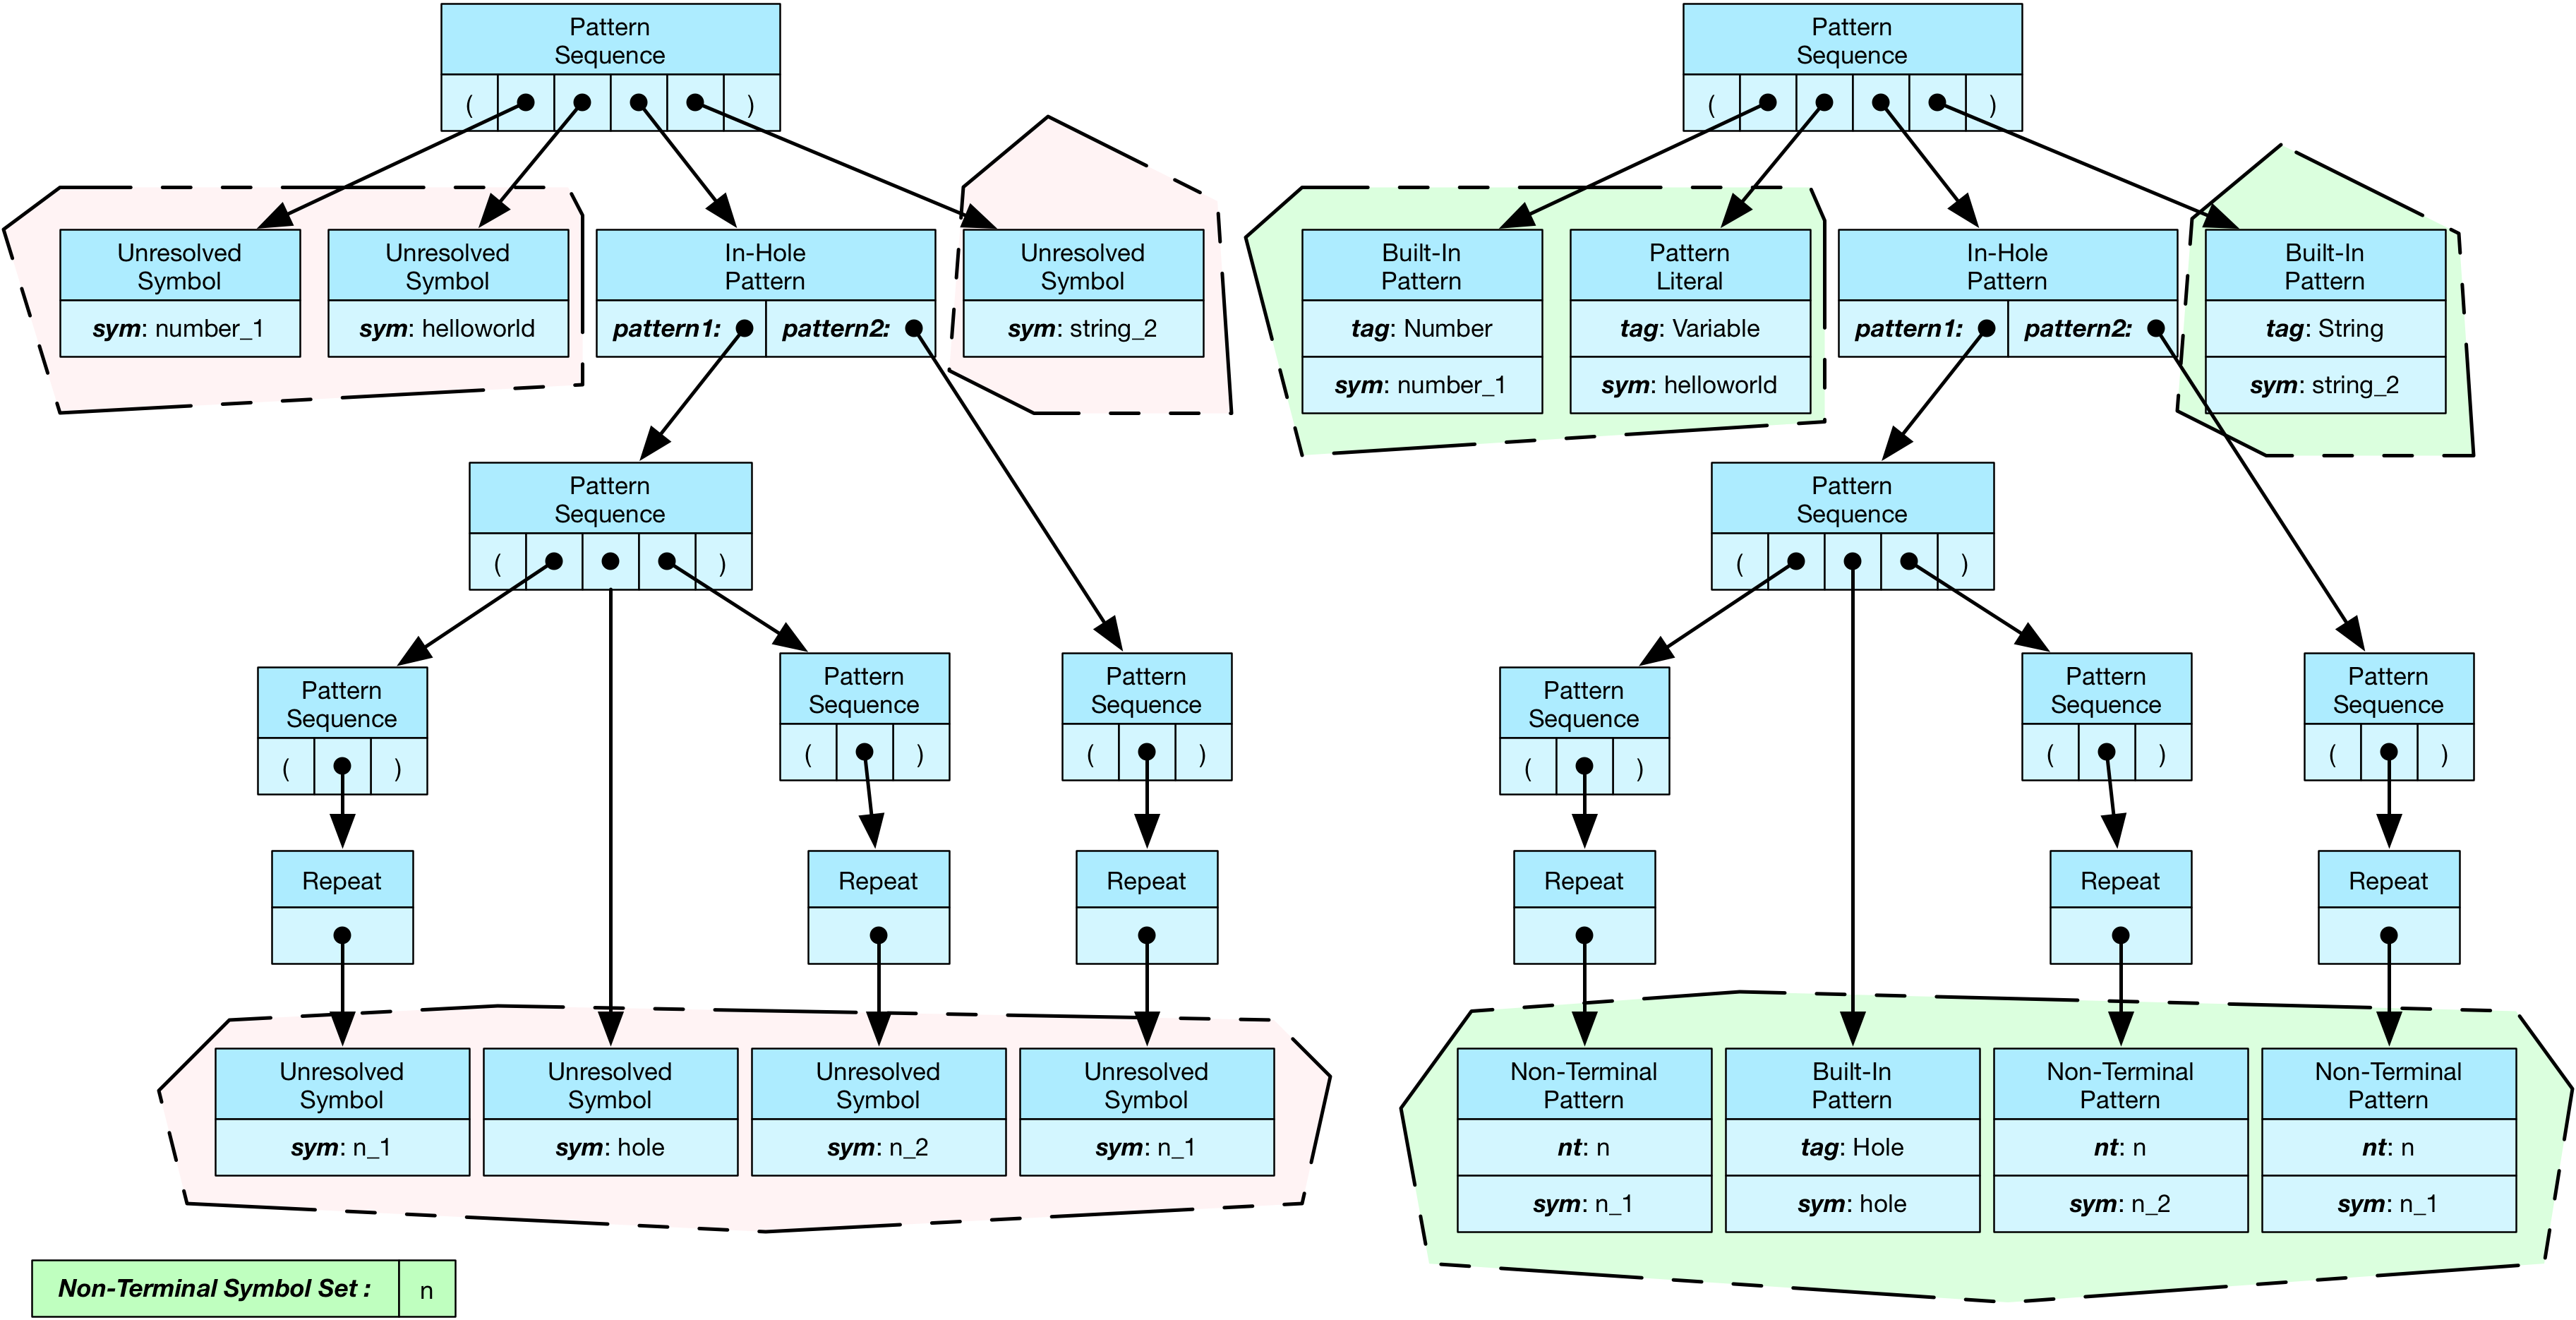
\includegraphics[scale=0.13]{transformation-pattern-resolvesym.png}
	}
\caption{Pattern before and after pattern variable resolution.}
\label{transformation-pattern-resolvesym}
\end{figure}

Figure \ref{transformation-pattern-resolvesym} shows an effect of transformation on pattern \texttt{(number\_1\ helloworld\ (in-hole\ ((n\_1\ ...)\ hole\ (n\_2\ ...))\ (n\_1\ ...))\ string\_2)}. Assume the related \texttt{define-language} has a single non-terminal \texttt{n}. Initially the pattern has six unresolved symbols - \texttt{number\_1}, \texttt{helloworld}, \texttt{n\_1}, \texttt{n\_2}, \texttt{hole} and \texttt{string\_2}. \texttt{number\_1}, \texttt{string\_2}, and \texttt{hole} become \texttt{BuiltInPattern} with appropriate tags,  \texttt{n\_1} and \texttt{n\_2} turn into non-terminals because prefix \texttt{n} is in the set of non-terminal symbols of given \texttt{define-language} and \texttt{helloworld} becomes a \texttt{LiteralPattern} with tag \texttt{Variable}. If this pattern were a part of \texttt{define-language}, \texttt{helloworld} would have been included into set $V$.

\section{DefineLanguage: Identifier Rewriting}
\label{section:id-rewrite}

\subsection{Motivation}

For patterns in the \DefineLanguageNoArg \space constraint checking is not performed. This means that in this context, patterns \texttt{(+ e e)} and \texttt{(+ e\_1 e\_1)} are equivalent. Due to design of \texttt{Match} class described in Section \ref{section:Match}, PyPltRedex needs to modify all such pattern-variables to be unique. Given the pattern-variable $pv$, $\mathit{prefix_{pv}}$ (defined in Section \ref{section:pv-resolve}) is extracted and concatenated with some previously unused integer - $\mathit{freshint()}$.

\subsection{Algorithm}
Given \LetDefineLanguage{$l$}, each pattern $p_i$ in \NtDefinitionN \space is visited recursively.
\begin{itemize}
\item Given \BuiltInPattern, \\ return \BuiltInPattern[$\mathit{tag}$][$\mathit{prefix_{pv}+freshint()}$][false].
\item Given \NonTerminal, \\ return \NonTerminal[$\mathit{nt}$][$\mathit{prefix_{pv}+freshint()}$][false].
\end{itemize}

\subsection{Example}

Figure \ref{id-rewrite-example} shows an example of the transformation on the \DefineLanguage form. Numerical suffixes are added to each occurrence non-terminal \texttt{e}, \texttt{n} and built-in pattern \texttt{number}.

\begin{figure}[h]
	\begin{minipage}{0.5\linewidth}
		\centering
		\begin{minted}[tabsize=2,obeytabs,escapeinside=||,mathescape=true,fontsize=\small]{Racket}
(define-language L
	(e ::= (+ |\colorbox{identbefore}{e} \colorbox{identbefore}{e}|)
	       (* |\colorbox{identbefore}{e} \colorbox{identbefore}{e}|) |\colorbox{identbefore}{n}|)
	(n ::= |\colorbox{identbefore}{number}|))
		\end{minted}
	\end{minipage}
	\begin{minipage}{0.5\linewidth}
		\centering
		\begin{minted}[tabsize=2,obeytabs,escapeinside=||,mathescape=true,fontsize=\small]{Racket}
(define-language L
	(e ::= (+ |\colorbox{identafter}{e\_0} \colorbox{identafter}{e\_1}|)
	       (* |\colorbox{identafter}{e\_2} \colorbox{identafter}{e\_3}|) |\colorbox{identafter}{n\_0}|)
	(n ::= |\colorbox{identafter}{number\_0}|))
		\end{minted}
	\end{minipage}
	\caption{\texttt{define-language} before and afte renaming of identifiers.}
	\label{id-rewrite-example}
\end{figure}

\section{Pattern: Ellipsis Depth Checking}

\subsection{Motivation}

Pattern-variables with the same symbol should be under a consistent number of ellipses. For example, in pattern \texttt{(((n\_1 ...)\ n\_1)\ ...)} the pattern variable \texttt{n\_1} is not under a consistent number of ellipses - one ellipses has an \textit{ellipsis depth} of one, whereas the other is two. Such invalid patterns should be reported during the compilation process.

In addition, after pattern matching, the pattern-variables are plugged into term-templates and the ellipsis depth of each pattern-variable is needed to ensure that a given term-template is well-formed.

\subsection{Algorithm}

During pattern traversal, the following need to be maintained:

\begin{enumerate}
\item
Let $n$ be \textbf{number of ellipses} on the path from the root of the pattern to some child sub-pattern. $n$ is modified accordingly when visiting patterns of kind \RepeatNoArg.

\item Association between pattern-variable $pv$ and its ellipsis depth $d$. Let $E=\emptyset$ containing pairs $(pv, d)$.
\end{enumerate}

Given some pattern $p$, \Visit{$p$}. The following kinds of $p$ are of interest.
\begin{itemize}
\item $p=$\space \PatternRepeat. Let $n=n+1$, \Visit{$p_r$}, and then let $n=n-1$.
\item $p=$\space \BuiltInPattern. Check if there exists a pair $(pv, d) \in E$. If it does not, $E = E \cup \{ (pv, d) \}$. Otherwise, if $n \neq d$, then $pv$ has inconsistent ellipsis depth and an Exception is raised.
\item $p=$\space \NonTerminal \space is handled in the same way as \BuiltInPatternNoArg.
\end{itemize}

Finally, the pattern $p$ has to be annotated with $E$ - \MakeAnnotation{$p$}{"EllipsisDepths"}{$E$}.

\section{DefineLanguage: Non-Terminal Cycle Checking}

\subsection{Motivation}
PltRedex doesn't allow language definitions such as the one in Figure \ref{dl-ntcyclegraph}.

\begin{figure}[H]

	\centering
\begin{minipage}{0.45\linewidth}
\begin{minted}[tabsize=1,obeytabs,escapeinside=||,mathescape=true,linenos,fontsize=\small]{racket}
(define-language L
	(e ::= (e e) n)
	(n ::= (n n) number p)
	(p ::= (p p) real e))
	(s ::= string)
\end{minted}
\end{minipage}
\begin{minipage}{0.45\linewidth}
	\centering
	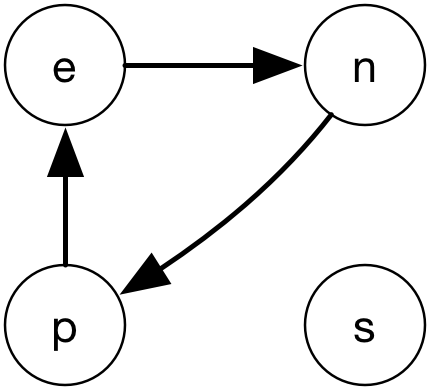
\includegraphics[scale=0.18]{transformation-pattern-ntgraph.png}
\end{minipage}
	\caption{\texttt{define-language} and its non-terminal graph}
	\label{dl-ntcyclegraph}
\end{figure}

The problem with the language above (aside from it being completely useless) is a cycle of non-terminals $n \rightarrow p \rightarrow e$. When testing if some term is a non-terminal, a term is matched against every pattern in a non-terminal definition. For example, given term \texttt{String("hello world")}, it is matched against non-terminal \texttt{e}. Since  the term doesn't match the pattern \texttt{(e e)}, non-terminal \texttt{n} is then matched. Since the term doesn't match any patterns here either, non-terminal \texttt{p} is then matched. Similarly, the term doesn't match any patterns here either, \texttt{e} is then matched, but that's where the matching has started and thus \textit{infinite recursion} becomes an issue. Languages need to be analyzed for presence of non-terminal cycles.

\subsection{Algorithm}
To detect such cycles, \DefineLanguageNoArg \space needs to be interpreted as a directed graph and some cycle-detecting algorithm must be used. The graph is constructed in the following manner.

\begin{enumerate}
\item
For each \NtDefinitionN[n], create a vertex labeled $n$.
\item
For $p_1, ..., p_n$, if $p_i$ is \NonTerminal[m][m\_?], create the edge $n\rightarrow m$.
\end{enumerate}


To detect cycles, depth-first-search is employed. Vertices in the graph can be assigned one of three colors:

\begin{itemize}
\item

\textbf{White} - meaning the vertex hasn't been visited before. All vertices are initially assigned this color.

\item
\textbf{Gray} - meaning successors of the vertex $v$ are still being visited. When $v$ is visited for the first time, $color(v)$ becomes \textbf{Gray}.
\item
\textbf{Black} - meaning all successors of the vertex $v$ have been explored.
\end{itemize}

A path of vertices visited during depth-first traversal is maintained.  Let $V$ be a set of vertices whose \DFSColor{$v$}{Black}, initially empty; let $U$ be a set of vertices whose \DFSColor{$v$}{White}, initially containing all vertices of the graph.

The algorithm proceeds in the following way:

\begin{enumerate}
\item Pick random vertex $u \in U$.
\item If \DFSColor{$u$}{White}, set color to \textbf{Gray} and add $u$ to the path.
\item If \DFSColor{$u$}{Gray}, report the cycle (using vertices on the path) and abort compilation.
\item Visit each successor vertex $u^{\prime}$ of $u$ recursively.
\item Set color of $u$ to \textbf{Black} and remove it from the path. $V = V \cup \{u\}$.
\item If there are no more vertices left to visit, let $U = U-V$ and go to step 1.
\end{enumerate}

It should be noted that the algorithm described does not report all the cycles in the graph but the first one it manages to find. One improvement could be finding all cycles in the graph.

%\section{Hole Reachability}

The pattern \InHolePattern requires $p_1$ to match exactly one \lstinline{hole} term. The main problem is counting a number of holes matched by non-terminal symbols of the language. Consider the language \lstinline{MatchesManyHoles} listed below.

\begin{lstlisting}
(define-language MatchesManyHoles
	(n ::= number)
	(P ::= E (n ... E ...))
	(E ::= (+ E P) (+ n E) hole))
\end{lstlisting}

To compute value for  the non-terminal \lstinline{E}, an analysis of pattern \lstinline{(+ E P)} is required but the value of \lstinline{E} is not yet known. Moreover, computing a single value that represents number of holes is insufficient; pattern lstinline{(E ...)} may match zero or many holes. Thus, a \textbf{minimum} and \textbf{maximum} number of holes matched by some pattern must be computed.

\subsection{Graph Modeling}

Graph consists of two parts - \textbf{outer-nodes} and \textbf{inner-nodes}.

Outer-nodes are a stand-in for the pattern and come in four different varieties:

\begin{itemize}
\item \lstinline{Sequence} representing pattern-sequences.
\item \lstinline{Repeat} representing ellipses.
\item \lstinline{LeafHole} representing the pattern \lstinline{hole}.
\item \lstinline{LeafNotHole} representing any other pattern except \InHolePattern
\end{itemize}

Inner-nodes are stored in \lstinline{Sequence} and \lstinline{Repeat} outer-nodes and act as non-terminal references. Each inner-node has a set of outer-node successors pointing to a set of expressions that the non-terminal matches.

Graph for language defined above can be seen in the following figure:
TODO

\subsection{Graph Construction}

Constructing the graph involves two stages:
\begin{enumerate}
\item
Creation of outer nodes for each top-level pattern such as `(+ E P)` or `hole`.
\item
Creation of inner nodes and edges from inner to outer nodes. If the outer node is a `Sequence` and it contains other sequences or ellipses, additional creation of outer-nodes will be required.
\end{enumerate}


\subsection{Creation of Outer Nodes}

A mapping of `M` has to be maintained between patterns in non-terminal definition. For each non-terminal definition `N` let `E\_N = \{\}` be a set storing top-level non-terminal references. For example, in the language described above for non-terminal definition `P` the only such reference is `E`.

Each non-terminal definition `N` is visited and we may come across the following patterns.
\begin{itemize}

\item
\BuiltInPattern. If kind is `Hole` then `n = LeafHole` node is created.  Otherwise, `n = LeafNotHole` node is created. Thus, `M = M union {(p, n)}`.
\item
\Nt. This means that `N` is also `nt` and thus all expressions in non-terminal definition of `nt` should also be reachable from any inner-node that reaches expressions in `N`. Thus, `E\_N = E\_N union {nt}`.
\item
\InHolePattern. Raise compilation error and quit. This, however, is not actual behavior of the PltRedex. (TODO explain why we handle it differently?)
* `p = PatternSequence(pattern ...)`. If length of `p` is zero, then `n = LeafNotHole`, otherwise `n = Sequence`. Thus, `M = M union {(p, n)}`.
\end{itemize}

Note that creating multiple `LeafHole` or `LeafNotHole` nodes is not necessary and existing nodes of these kinds can be reused. This means that the graph may have at most two leaf nodes.


\subsection{Creation of Inner Nodes and Edges}

The only top-level pattern kind that may contain inner nodes at this point is `Sequence` and thus they need to be visited. One thing that needs to be maintained is the stack `S` of outer-nodes where inner-nodes are to be stored.

For each non-terminal definition `N` and each pattern $p_i$, if $p_i$ is `PatSequence`, retrieve `M[$p_i$]` from the mapping and place on top of the stack S. For each subpattern $q_i$ in $p_i$, visit $q_i$.

\begin{itemize}
\item
\PatternSequence. Create outer-node `Sequence` `s` for `p`; create inner node `i`; add edge `i->s`. Retrieve parent outer-node `O` and add node `i` to it. Append `s` to the stack `S`. For each child pattern $c_i$ of `p`, recursively visit each $c_i$. Pop topmost element off the stack `S`.

\item
* \Repeat. Create outer-node `Repeat` `r` for `p`, create inner node `i`, add edge `i->r`. Retrieve parent outer-node `O` and add node `i` to it. Append `r` to the stack `S`. Visit child pattern `c` of `p`. Pop topmost element off the stack `S`.

\item
\InHolePattern Raise compilation error and quit.

\item
\BuiltInPattern. Create inner node `i`. If kind is Hole then let s = LeafHole, otherwise s = LeafNotHole. Create edge `i->s`.  Retreieve parent outer-node `O` from the top of the stack and add node `i` to it.

\item
\Nt Create inner node `i`. For each pattern in non-terminal definition of `nt`, retrieve outer-node `o` from the mapping `M` and create edge `i->o`. Do the same for each non-terminal in the set `E\_nt`. Retrieve outer-node `O` from the stack and append `i` to it.

\end{itemize}

\subsection{Minimal/Maximal Value Representation and Arithmetic}

Minimum / maximum number of holes can be one of the following: `Zero`, `One`, `Many` (i.e. >= 2) and `Uninitialized` indicating said value should not be used for computation just yet.

Furthermore, three operators need to be defined - `+`, `min`, `max`. Assume Zero = 0, One = 1, Many = 2 and Uninitialized = 3

Addition operation.

\begin{align}
	a + b =
	\begin{cases}
		3 \text{ if } a = 3 \text{ and } b = 3 \\
		a \text{ if } b = 3 \\
		b \text{ if } a = 3 \\
		min(a + b, 2)
	\end{cases}
\end{align}

Min operation:

\begin{align}
	min(a,b) =
	\begin{cases}
		3 \text{ if } a = 3 \text{ and } b = 3 \\
		a \text{ if } b = 3 \\
		b \text{ if } a = 3 \\
		min(a, b)
	\end{cases}
\end{align}

Max operation:
\begin{align}
	max(a, b) =
	\begin{cases}
		3 \text{ if } a = 3 \text{ and } b = 3 \\
		a \text{ if } b = 3 \\
		b \text{ if } a = 3 \\
		max(a, b)
	\end{cases}
\end{align}


\subsection{Computation of Values}
Min/max values are computed both for inner-nodes and outer-nodes. First, they have to be initialized.

\begin{itemize}
\item
Inner nodes are initialized with (Uninitialized, Uninitialized)
\item
`Sequence` and `Repeat` outer nodes are initialized with (Uninitialized, Uninitialized)
\item
`LeafHole` outer node is initialized with (One, One)
\item
`LeafNotHole` outer node is initialized with (One, One)
\end{itemize}


Given initial values $min_inner$, $max_inner$ of some inner-node  and new values $v_1$, $v_2$, $min_inner = min(min_inner, v1)$, $max_inner = max(max_inner, v2)$.


Given outer-node `o`, there are a few cases to consider.

\begin{itemize}
\item
`LeafHole` and `LeafNotHole` - its min/max values are never updated.
\item
* `Sequence` - $min_o = \sum_{i in inner(o)} min_i$ and $max_o = \sum_{i in inner(o)} max_i$. Summation is described above.
\item
* `Repeat` - $min_o = Zero$, $max_o = Many if max_inner = One or max_inner = Many else Zero$.
\end{itemize}

\subsection{Hole Reachability Algorithm}

Before initiating graph traversal, verify if `LeafHole` node is actually in `V`. If there is no such node, that means the source pattern does not match any `hole` and thus each non-terminal should be annotated with `Zero,Zero` number of holes.

Otherwise, the graph is traversed in reverse direction starting from nodes `LeafHole` and `LeafNotHole` using breadth-first strategy. Maintain queue Q that initially stores all `LeafHole` and `LeafNotHole` nodes.

The algorithm is as follows:
\begin{enumerate}
\item
Remove outer node `o` from the queue `Q`.
\item
* For each inner-node `i` such that `i->o`:
	\begin{enumerate}
	\item
	if `parent(i) = o` then $update(i, o_min, o_max)$ and `update(o)`. This means that if the inner node contains an edge to the outer-node `o` `i` is a child of, thus can be considered a "self-loop". The reason for doing this will be discussed later. (TODO is this actually needed aside from really degenerate patterns?)
	\end{enumerate}

\item
For each inner-node `i` such that `i->o`:
	\begin{enumerate}
	\item
	if `parent(i) != o`, $update(i, o_min, o_max)$ and update(o). If values of $o_min, o_max$ are different from ones before update operation, add `o` to the queue `Q`.
	\end{enumerate}

\item
* Repeat until queue `Q` is empty.

\end{enumerate}


\subsection{Computing Min/max values for non-terminal definition}

Given non-terminal definition `nt` and set of patterns `P` it matches, $min_nt = max_nt = Uninitialized$. Then, $min_nt = \min_{i in P} min_i$ and $max_nt = \max_{i in P} max_i$.Note that some parrern `i` in `P` may be Nt, in which case $min_i$ and $max_i$ for non-terminal definition `i` first. By ensuring that language contains no non-terminal cycles, such recursive procedure s guaranteed to terminate.

After completing all computations, each non-terminal definition `nt` is annotated with corresponding $min_nt, max_nt$.


\subsection{Edge cases}.

This algorithm doesn't do one very specific thing - infinite terms and presence of `hole`. Consider the language below

\begin{lstlisting}
(define-lagnuge Infinite
     (P ::= (E))
     (E ::= P hole))
\end{lstlisting}

\subsection{Example}
TODO

%\section{Pattern: \lstinline{in-hole} Pattern Checker}

Having computed `min/max` numbers for each non-terminal in the language, now the question is whether `pattern1` in pattern \InHolePattern actually matches exactly one hole. Doing so involves two stages:

\begin{enumerate}
\item
Locating \InHolePattern in the top-level pattern.
\item
Checking if $p_1$ matches exactly one hole. Since $pattern1$ doesn't necessarily have to be a non-terminal, extra work will be required.
\end{enumerate}

\subsection{Checking pattern for number of holes}

Assuming \InHolePattern pattern has already been found, $p_1$ has to be visited recursively. One of the following nodes may be visited.

\begin{itemize}
\item
\BuiltInPattern - if $t=$hole then $min_p = One, max_p = One$, otherwise $min_p = Zero, max_p=Zero$.

\item
\Nt. Read appropriate annotation from non-terminal definition in `define-language` and return values.

\item

\LiteralPattern min\_p = Zero, max\_p = Zero.

\item
\InHolePattern. Return $min_p = Zero, max_p = Zero$, this seems to be default PltRedex behaviour.

\item
\Repeat. Recursively visit the $p$ obtaining $min_p2$, $max_p2$. The logic for Repeat is identical to the one used in **Hole Reachability**; that is:
	\begin{itemize}
	\item
	$min_n = Zero$
	\item
	$max_p = Many if max_p2 = One or max_p2 = Many$
	\item
	$max_p = Zero$ otherwise
	\end{itemize}

\item
* \PatternSequence. Initially, $min_p$, $max_p = Unitialized$. Then, $min_p = \sum_{p_i in p} minp_i$. To obtain $minp_i$, $p_i$ has to be recursively visited.
\end{itemize}

\subsection{Example}
TODO

\section{Pattern: Constraint Check Insertion}
\label{section:constraint-check}
\subsection{Motivation}
As mentioned before, PLTRedex supports a few different forms of constraint checking; however, for the initial PyPltRedex implementation only the "equality of terms" constraint check is supported. For example, in the pattern \texttt{(number\_1 number\_1)} both terms bound to \texttt{number\_1} must be the same, meaning the term \texttt{(1 1)} does match the pattern but \texttt{(1 2)} does not.

However, since the current design of the \texttt{Match} class, explained in Section \ref{section:Match}, does not allow assigning multiple terms to the same pattern-variable, certain pattern-variables have to be renamed. Given $n$ occurrences of a pattern-variable, $n-1$ occurrences are to be renamed. After completion of pattern matching these $n-1$ pattern-variables must be removed from all returned \texttt{Match} instances.

Finally, actual equality checks have to be inserted. There are two obvious strategies that could be employed:

\begin{itemize}
\item Compare required pattern-variables \textit{after} matching a term against a pattern. The disadvantage of this strategy is that the pattern has to be matched entirely despite the fact that failure may happen very early in the matching process, thus resulting in useless work.

\item Compare required pattern-variables at the \textit{earliest} time possible, as pattern-variables become available. This is the strategy that PyPltRedex uses.
\end{itemize}

\subsection{Pattern-Variable Renaming}
Pattern variable $pv$ is renamed in the following manner: $\mathit{pv + \# + freshint()}$, $\mathit{freshint()}$ if $\mathit{freshint() > 0}$ otherwise $pv$. $\mathit{freshint}$ operation was defined previously in Section \ref{section:id-rewrite}. For example, assuming $\mathit{freshint()=0}$, renaming \texttt{m} results in \texttt{m}. Successive application of the renaming operation results in \texttt{$m\#1$}.

\subsection{Algorithm}
Since the algorithm is based on renaming (or modification) of pattern-variables, let $v^{\prime}$ be a new pattern-variable after modifying $v$. The pairs $(pv, pv^{\prime})$ need to be maintained in order to decide where to insert equality checks. Let $M$ be a set containing such pairs. Furthermore, to remove renamed pattern-variables after matching, the set $R$ containing such pattern-variables has to be maintained.

Given some pattern $p$, \Visit{$p$}. The following kinds of $p$ are of interest.
\begin{itemize}
\item $p=$\space \BuiltInPattern. Let $pv^{\prime}$ be a renamed variable and let $M=\{(pv, pv^{\prime})\}$. If $pv \neq pv^{\prime}$, $R=R \cup \{pv^{\prime}\}$. Return \BuiltInPattern[$tag$][$pv^{\prime}$][false] and $M$.
\item $p=$\space \NonTerminal. Let $pv^{\prime}$ be a renamed variable and let $M=\{(pv, pv^{\prime})\}$. If $pv \neq pv^{\prime}$, $R=R \cup \{pv^{\prime}\}$. Return \NonTerminal[$nt$][$pv^{\prime}$][false] and $M$.
\item $p=$\space \LiteralPattern \space contains no pattern-variables and thus $p$ and $\emptyset$ are returned.
\item $p=$\space \PatternRepeat. Let $p_r^{\prime}, M=$\space\Visit{$p_r$}. Return \PatternRepeat[$p_r^{\prime}$], $M$.
\item
$p=$\space \PatternSequence. If the sequence contains no child patterns, return $p$, $\emptyset$. Define \texttt{merge} operation that, given two sets $M_i, M_j$ returns two sets $M_k$ and $M_r$; this operation will be discussed below.
Let $p^{\prime}$ be the pattern sequence that replaces $p$.
Let $p_1^{\prime}, M_1$=\Visit{$p_1$}. Insert $p_1^{\prime}$ into $p^{\prime}$. For $p_i \in p_2, ..., p_n$, let $p_i^{\prime}, M_i$=\Visit{$p_i$}.
	\begin{enumerate}
	\item
	Insert $p_i^{\prime}$ into $p^{\prime}$.
	\item
	Let $M_1$, $M_r$ = \texttt{merge}($M_1$, $M_i$). For each pair of pattern-variables $(pv_a, pv_b) \in M_r$, insert \PatternCheckConstraint[$pv_a$][$pv_b$][false] into $p^{\prime}$.
	\end{enumerate}
Finally, return $p^{\prime}, M_1$.

\item
$p=$\space \PatternInHole.\\ Let $p_1^{\prime}, M_1$= \Visit{$p_1$} and $p_2^{\prime}, M_2$= \Visit{$p_2$}. Let $M, M_r$=\texttt{merge}($M_1$, $M_2$). For each pair of pattern-variables $(pv_a, pv_b) \in M_r$, let $c_i$=\PatternCheckConstraint[$pv_a$][$pv_b$][false]. Return \PatternInHole[$p_1^{\prime}$][$p_2^{\prime}$][$c_1$][$c_n$][false], $M$.
\end{itemize}

Finally, make an annotation \MakeAnnotation{$p$}{"PatConstraintCheckRemoveVars"}{$R$}.

\subsection{\texttt{merge} Operation}
Before proceeding with pattern traversal, \texttt{merge} operation needs to be defined. Given two sets $M_1$ and $M_2$ it produces two sets $M$ and $M_r$. Those sets are constructed in the following manner:

\begin{enumerate}
\item Let $M=\emptyset$ and $M_r=\emptyset$.
\item For each $(pv, pv^{\prime}) \in M_1$, find a pair $(pv, pv^{\prime\prime}) \in M_2$.
\begin{enumerate}
\item If such pair exists, then $M_r=M_r \cup \{(pv^{\prime},  pv^{\prime\prime})\}$ and $M=M \cup \{(pv,  pv^{\prime\prime})\}$.
\item Otherwise, $M=M \cup \{(pv,  pv^{\prime})\}$
\item For any other $(pv, pv^{\prime\prime}) \in M_2$ s.t.  $(pv, pv^{\prime}) \notin M_1$, $M=M \cup \{(pv,  pv^{\prime\prime})\}$
\end{enumerate}
\end{enumerate}

\subsection{Example}

\begin{figure}[htp]
	\centering
	\makebox[\textwidth][c] { 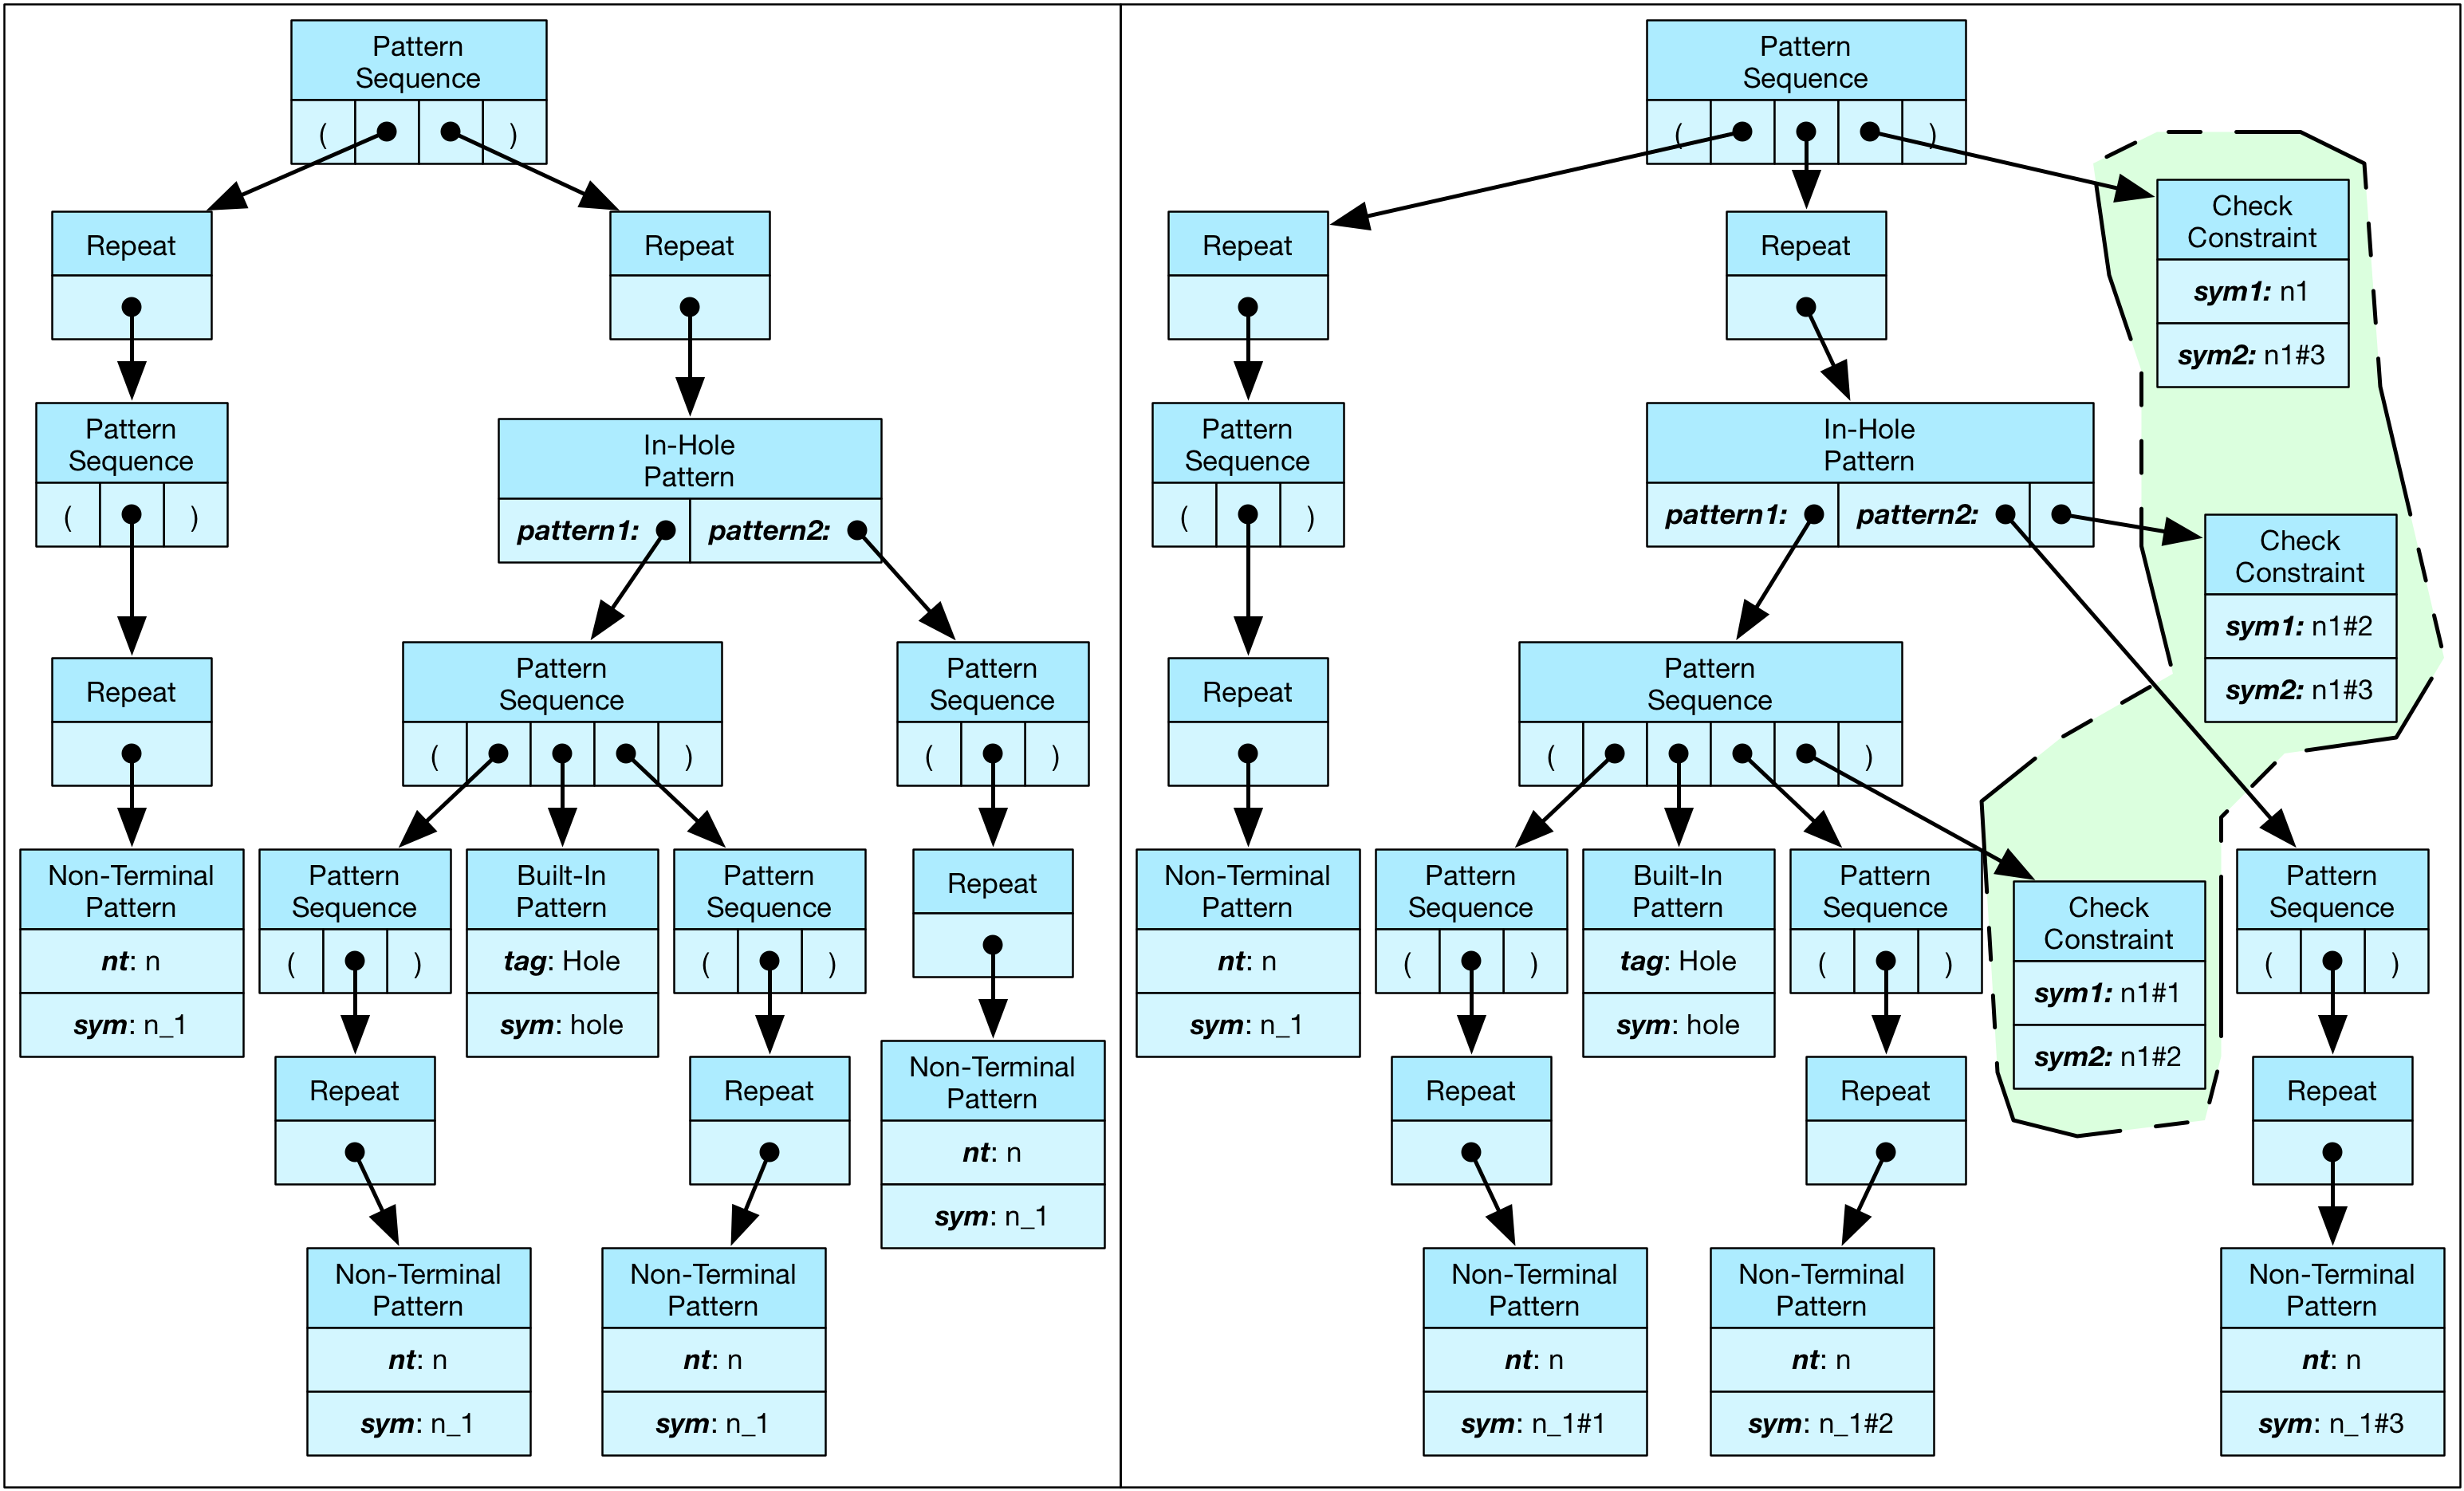
\includegraphics[scale=0.135]{transformation-pattern-constraintcheck.png} }
\caption{Applying transformation to pattern \texttt{((n\_1\ ...)\ ...\ (in-hole\ ((n\_1\ ...)\ hole\ (n\_1\ ...))\ (n\_1\ ...))\ ...)}, before and after.}
\label{transformation-pattern-constraintcheck}
\end{figure}

Figure \ref{transformation-pattern-constraintcheck} shows an effect of described transformation on the pattern \texttt{((n\_1\ ...)\ ...\ (in-hole\ ((n\_1\ ...)\ hole\ (n\_1\ ...))\ (n\_1\ ...))\ ...)}. Notice that all occurrences of \texttt{n\_1} have an ellipsis depth of two. The first occurrence of \texttt{n\_1} goes unmodified. Then, when processing the first pattern inside the \texttt{in-hole} pattern, there are two occurrences of \texttt{n\_1}. The first occurrence is renamed to \texttt{n\_1\#1}, the second to \texttt{n\_1\#2}, and \texttt{CheckConstraint(n\_1\#1, n\_1\#2)} is appended to the \texttt{PatternSequence}. The final occurrence of \texttt{n\_1} is seen in the second pattern of \texttt{in-hole} and is renamed to \texttt{n\_1\#3}. \texttt{CheckConstraint(n\_1\#2, n\_1\#3)} is then added to the \texttt{in-hole}. Finally after exiting \texttt{in-hole}, \texttt{CheckConstraint(n\_1, n\_1\#3)} is appended to \texttt{PatternSequence}.

\section{Pattern: Pattern-Variable Extraction}
\label{section:pv-extraction}

\subsection{Motivation}
Since \texttt{Match} instances are initialized with pattern-variables, all pattern-variables used by some pattern $p$ need to be known. 

\subsection{Algorithm}
The algorithm recursively traverses the pattern and at each step returns a set of pattern-variables $V$. Given some pattern $p$, $V=$\space \Visit{$p$}. The following kinds of $p$ are of interest.

\begin{itemize}
\item $p=$\space \NonTerminal. Return $V = \{ pv \}$.
\item $p=$\space \BuiltInPattern. Return $V=\{ pv \}$.
\item $p=$\space \LiteralPattern. Return $V=\emptyset$.
\item $p=$\space \PatternSequence. Return $V=\bigcup_{i=1}^{n}$\Visit{$p_i$}.
\item $p=$\space \PatternRepeat. Let $V_r=$\space\Visit{$p_r$}. Need to annotate $p$ with $V_r$: \MakeAnnotation{$p$}{"PatternVariables"}{$V_r$}.
\item $p=$\space \PatternInHole. Let $V_1=$\space\Visit{$p_1$} and  $V_2=$\space\Visit{$p_2$}. Annotate $p_1$ and $p_2$ with corresponding pattern-variable sets: \MakeAnnotation{$p_1$}{"PatternVariables"}{$V_1$} and \\ \MakeAnnotation{$p_2$}{"PatternVariables"}{$V_2$}. Return $V = V_1 \cup V_2$.
\end{itemize}

Finally, \MakeAnnotation{$p$}{"PatternVariables"}{$V$}.

\section{Term-Template: Ellipsis Depth Checking}

\subsection{Motivation}

Immediately after parsing the PLTRedex specification, it is unknown whether certain elements of a term-template are pattern-variables or just literal variables. These elements are represented with \UnresolvedSymbol \space instances. Since pattern-variables may be under ellipsis, all occurrences of the pattern-variable must have consistent \textit{ellipsis depths}. Finally, since ellipses produce lists of terms, it has to be decided how and where these sub-terms are to be extracted from the last and plugged into the term-template. An ellipsis depth of each pattern-variable is assumed to be known - it comes from \textbf{EllipsisDepths} annotation of related pattern $p$.

These goals are achieved by introducing the following term-template annotations. For term-template $t$,

\begin{itemize}
\item
\texttt{InArg(parameter\_name)} indicates that there is a pattern-variable in $t$ or child term-template of $t$ that requires substitution; the value of the term to be plugged in is assigned to meta-variable \texttt{parameter\_name}.
\item
\texttt{ReadMatch(parameter\_name, sym)} indicates that there is a pattern-variable in $t$ or child term-template of $t$ that requires substitution; the value of the term to be plugged in is read from provided \texttt{Match} instance by retrieving a term assigned to pattern-variable \texttt{sym} and assigning it to \texttt{parameter\_name}.
\item
\texttt{ForEach(parameter\_name)} annotation is added to \TermRepeat \\ term-templates. Assuming the term assigned to \texttt{parameter\_name} is a list, each term of that list is plugged into term-template $t_r$.
\end{itemize}

\subsection{Algorithm}

To perform annotation, a \textbf{path} of term-templates must be maintained to be able to count all occurrences of ellipsis on the path to the root term-template. The path is represented using a stack. When the term-template $t$ is visited, it is added to the top of the stack, child term-templates of $t$ are visited recursively and $t$ is popped from the stack. Now, \Visit{$t$}.
\begin{itemize}

\item
	$t=$\TermUnresolvedSymbol. First, check if the pattern-variable $\mathit{sym}$ is present in the set \textbf{EllipsisDepths}. If it is not, then $sym$ is just a literal variable and is resolved to \TermLiteral[Variable][$sym$][false].
Otherwise, $sym$ is a pattern-variable with \textit{expected ellipsis depth} $d_e$. Let $d_a$ be the \textit{actual ellipsis depth}, initially zero. Let $d_p$ be a number of \RepeatNoArg \space term-templates on the \texttt{path}. In the end it must be true that $d_p \geq d_e$ and $d_a = d_e$. There is a number of cases to consider. Let $x$ be a fresh symbol.
	\begin{itemize}
	\item
	$d_e=0$. Add the following annotation to $t$: \MakeAnnotation{$t$}{"MatchRead"}{$(n, sym)$} and return.
	\item
	$d_e>0$. Add the following annotation to $t$: \MakeAnnotation{$t$}{"InArg"}{$n$}. Now, contents of the \texttt{path} has to be inspected to be able to determine $d_a$. The topmost element of the \texttt{path} is $t$; iterate over the \texttt{path} in reverse order ignoring the topmost term-template. Let $t^{\prime}$ be a term-template on the \texttt{path}.
		\begin{enumerate}
		\item
		$t^{\prime}=$\space \texttt{TermSequence} or $t^{\prime}=$\space \texttt{InHole}; and $d_a \neq d_e$. Add the following annotation to $t^{\prime}$: \MakeAnnotation{$t^{\prime}$}{"InArg"}{$n$}.
		\item
		$t^{\prime}=$\space \texttt{TermSequence} or $t^{\prime}=$\space \texttt{InHole}; and $d_a = d_e$.  Add the following annotation to $t^{\prime}$: \MakeAnnotation{$t^{\prime}$}{"MatchRead"}{$(n, sym)$} and return.
		\item
		$t^{\prime}=$\space \RepeatNoArg. $d_a = d_a + 1$ and add the following annotation to $t^{\prime}$: \MakeAnnotation{$t^{\prime}$}{"ForEach"}{$n$}.
		\item
		$t^{\prime}=$\space \texttt{PythonCall}. This case doesn't happen.
		\end{enumerate}
	  Otherwise, all elements of the \texttt{path} have been inspected with $d_a \neq d_e$, meaning $d_p < d_e$. An \texttt{Exception} is raised.
	\end{itemize}
\item
$t=$\space \TermRepeat. Recursively \Visit{$t_r$}. By now $t$ must contain at least one \texttt{ForEach} annotation indicating that there's at least one pattern-variable under ellipsis. Raise \texttt{Exception} if that's not the case.
\item
$t=$\space \TermSequence. For $t_i$, recursively \Visit{$t_i$}.
\item
$t=$\space \TermInHole. \\ Recursively \Visit{$t_1$} and \Visit{$t_2$}.
\item
$t=$\space \PythonCall. Remove all elements $p_1, ..., p_m$ from \texttt{path} and recursively \Visit{$t_i$}. Push elements $p_1, ..., p_m$ to the \texttt{path}. Since \texttt{PythonCall} emulates escape to Racket, all term-templates $t_i$ must be self-contained and have valid ellipsis depths.
\end{itemize}

\section{Term-Template: Rewriting Metafunction Applications}

Since metafunction applications have the following shape:\newline \texttt{(metafunction-name\ term-template\ ...)} these can be detected quite trivially given a list of defined metafunctions. 

\subsection{Algorithm}
Let $Mf$ be the set of metafunction names. Let $t$ be some term-template, \Visit{$t$}. 
\begin{itemize}
\item $t=$\space \TermSequence. Check if $t_1$ is \TermLiteral\space with $kind=$\space Variable and $v \in Mf$. Return \\ \ApplyMetafunction[$v$][$t$][false] if that is the case, handling annotations as described below; otherwise return $t$. 

$t$ may contain \texttt{InArg} and \texttt{MatchRead} annotations and they are modified in the following way:
\begin{itemize}
\item
\texttt{InArg} annotations are left intact. Signatures of both \texttt{TermSequence} and \texttt{ApplyMetafunctions} must match.
\item
\texttt{MatchRead} annotations can be safely removed. None of such variable assignments are used to generate $t$.
\end{itemize}
\end{itemize}
\subsection{Example}
The example shown in Figure \ref{transformation-term-mfapply} displays the transformation described above given a set of meta-function names only containing a single \texttt{set-contains?}. Since the first element of \texttt{TermSequence} is a \texttt{Variable} term-template with suitable name, an additional \texttt{MetafunctionApplication} term is added.

\begin{figure}[htbp]
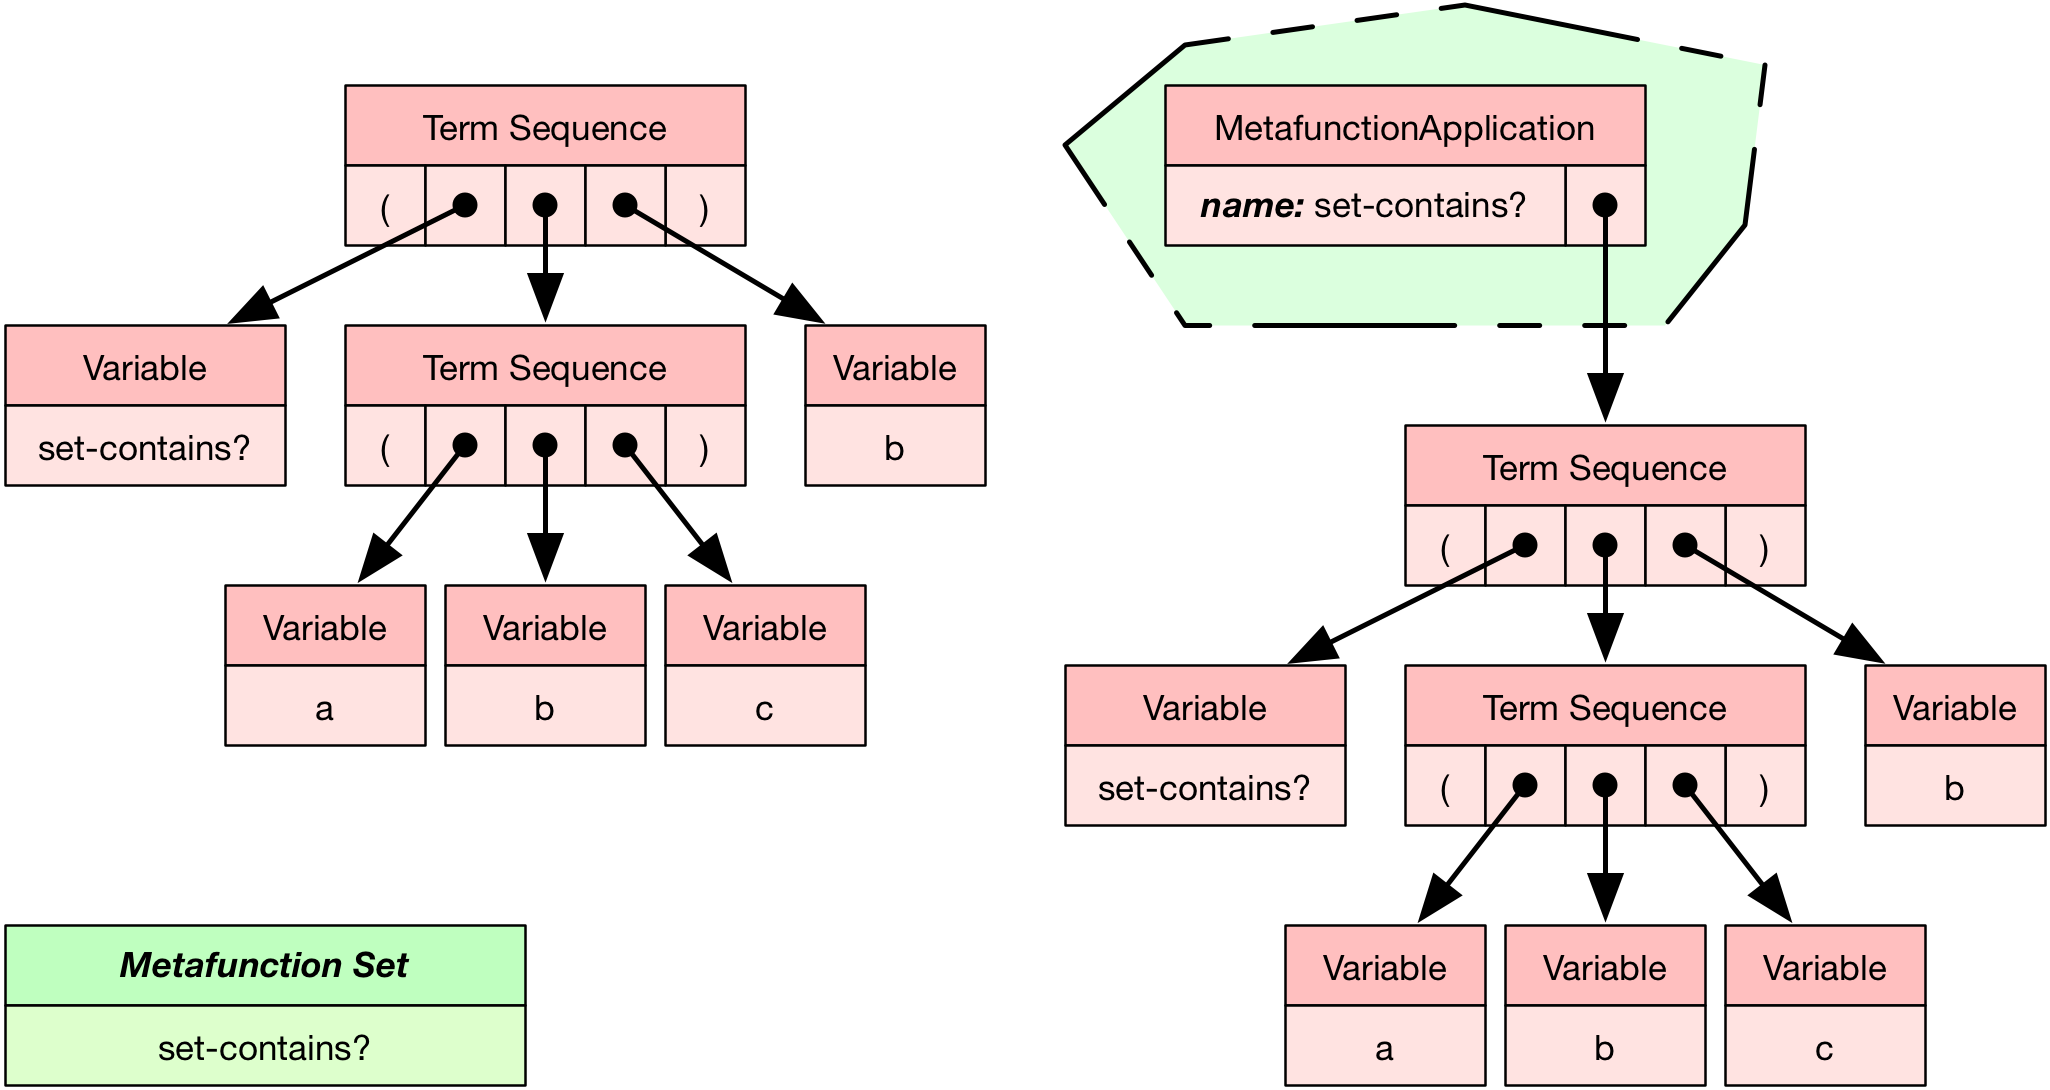
\includegraphics[scale=0.20]{transformation-term-mfapply.png}
\caption{Term-template before and after applying metafunctions.}
\label{transformation-term-mfapply}
\end{figure}

\section{Preprocessing Top-Level Forms}

Having defined and explained transformation/analysis passes for both patterns and term-templates, these are combined according to the needs of top-level forms. They are depicted in Figure \ref{transform-pipeline}. 

There are three different strategies that can be applied to patterns. Strategy \textbf{(a)} is applied to all patterns used in \texttt{define-language} form. Strategy \textbf{(b)} is applied to patterns used for domain/codomain testing of terms. Strategy \textbf{(c)} is applied to any other pattern. For term-templates, there's only a single transformation strategy.

\begin{figure}[ht]
\centering
	\makebox[\textwidth][c] { 
		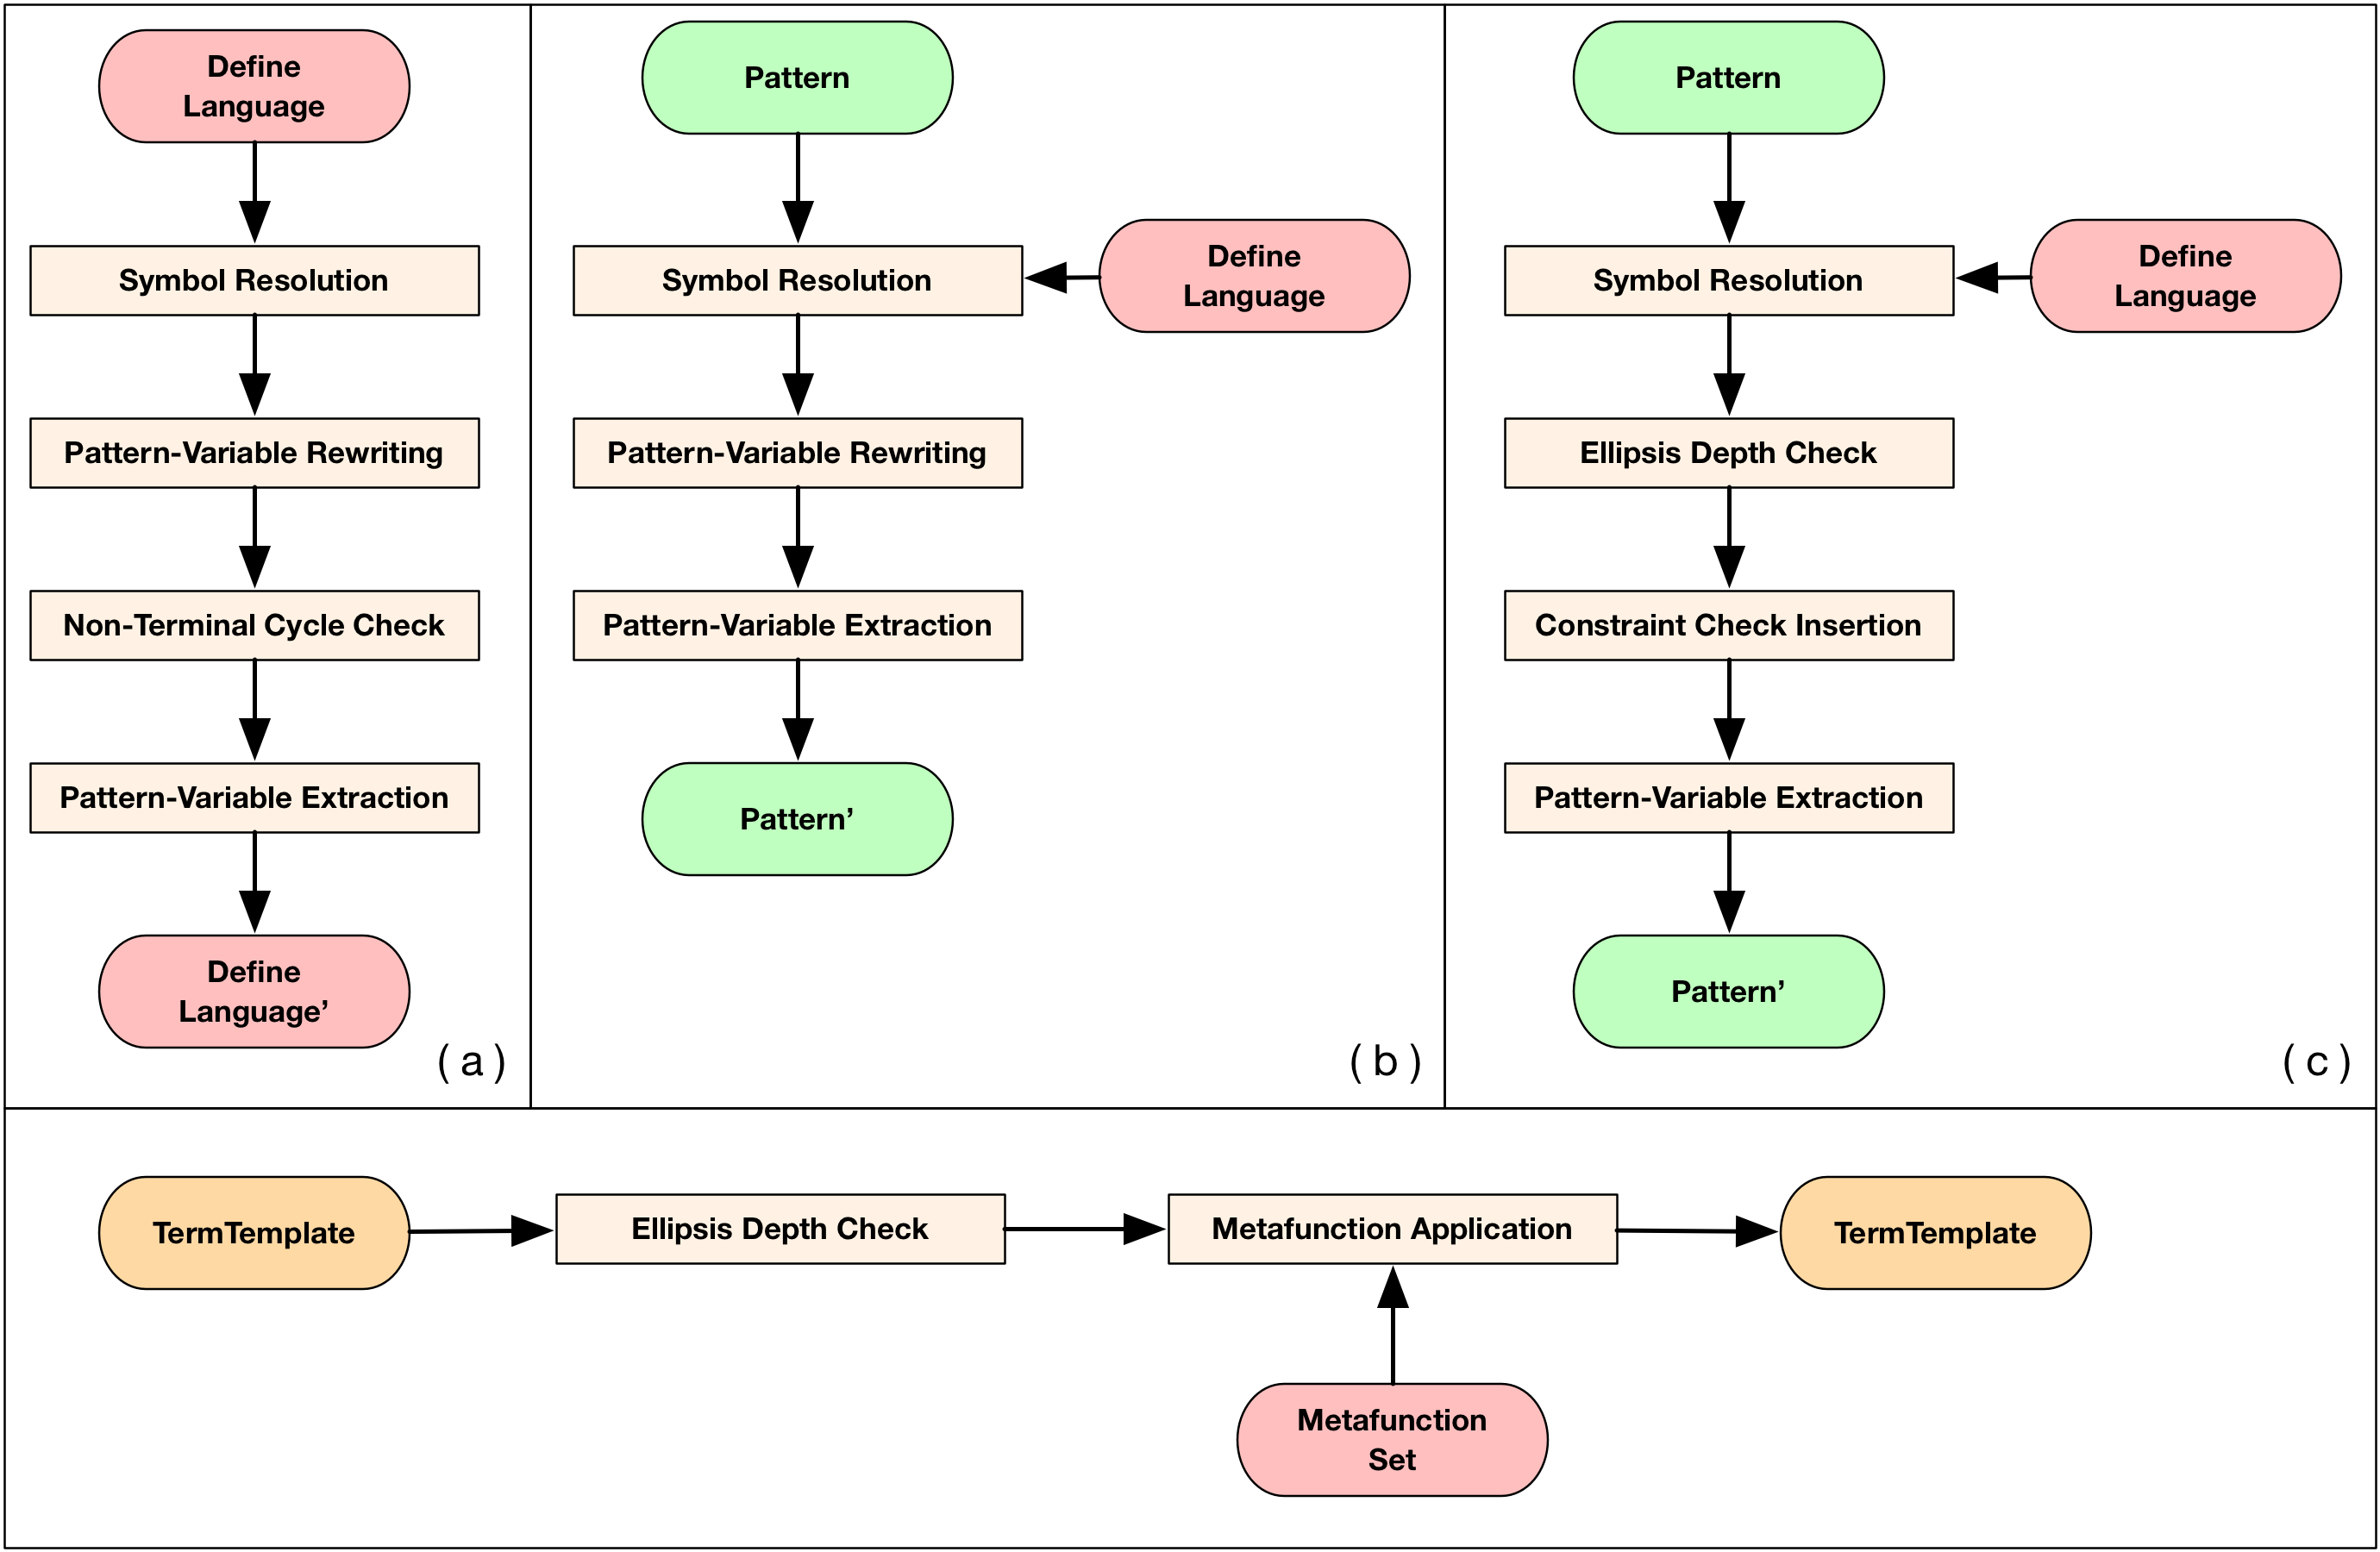
\includegraphics[scale=0.165]{transform-pipeline.png}
	}
	\caption{Transformations applied to patterns and term-templates.}
	\label{transform-pipeline}
\end{figure}


Notice that non-terminal resolution occurs with respect to non-terminal definitions on some \DefineLanguageNoArg \space form. Similarly, \textit{Metafunction Application} Pass requires the set $Mf$ containing all meta-functions defined until this point. 

\begin{enumerate}
\item All $tl=$\space \TlDefineLanguage \space forms. Maintain a set $L$ that stores ($n, tl$) pairs.
\item All $tl=$\space \TlDefineMetafunction \space forms. Maintain a set $M$ that stores $(n, tl)$ pairs.
\item All $tl=$\space \TlDefineReductionRelation \space forms. Maintain a set $R$ that contains $(n, tl)$ pairs.
\end{enumerate}

\subsection{Top-Level Form Analysis}

\begin{itemize}
\item
Given $tl=$\space \TlDefineLanguage
	\begin{enumerate}
		\item Apply strategy \textbf{(a)} to $tl$ resulting in $tl^{\prime}$.
		\item $L = L \cup \{ (n, tl^{\prime}) \}$
		\item Return $tl^{\prime}$.
	\end{enumerate}

\item $tl=$\space \TlDefineMetafunction:
	\begin{enumerate}
	\item Ensure that there exists a tuple $(l, df) \in L$, otherwise raise an Exception.
	\item Apply strategy \textbf{(b)} to $domain$ and $codomain$ patterns resulting in $domain^\prime$ and $codomain^\prime$.
	\item For each $mc_i=$ \MetafunctionCase, apply strategy \textbf{(c)} to $p$ thus resulting in $p^{\prime}$ and apply term-processing strategy to $t$ resulting in $t^{\prime}$. Let $mc_i^{\prime}$ = \MetafunctionCase[$p^{\prime}$][$t^{\prime}$].
	\item Let $tl^\prime$  = \TlDefineMetafunction[$n$][$l$][$domain^\prime$][$codomain^\prime$][$mc_1^\prime$][$mc_n^\prime$][false].
	\item $M = M \cup \{ (n, tl^\prime)\}$ and return $tl^\prime$.
	\end{enumerate}

\item $tl=$ \TlDefineReductionRelation:
\begin{enumerate}
\item Ensure that there exists a tuple $(l, df) \in L$ otherwise raise an Exception.
\item Apply strategy \textbf{(b)} to $domain$ pattern resulting in $domain^\prime$, if it exists.
\item For each $rc_i=$ \ReductionCase \space in $r$, apply strategy \textbf{(c)} to $p$ resulting in $p^{\prime}$ and apply the only term-processing strategy to $t$ resulting in $t^\prime$. Let $rc_i^\prime=$\space \ReductionCase[$p^{\prime}$][$t^{\prime}$][$n$][false].
\item Let $tl^\prime=$\space \TlDefineReductionRelation[$n$][$l$][$domain^\prime$][$rc_1^\prime$][$rc_n^\prime$]
\item $R = R \cup \{ (n, tl^\prime) \}$ and return $tl^\prime$.

\end{enumerate}

\item $tl=$ \ReadFromStdinAndApplyReductionRelation
\begin{enumerate}
\item If $f$ is present, ensure there exists a tuple $(f, mf) \in M$, otherwise raise Exception.
\item Ensure there exists a tuple $(r, red) \in R$, otherwise raise an Exception.
\item Return $tl$.
\end{enumerate}

\item
$tl=$ \RedexMatchAssertEqual.
	\begin{enumerate}
	\item Ensure that there exists a tuple $(l, df) \in L$, otherwise raise an Exception.
	\item Process $p$ according to strategy \textbf{(c)} resulting in $p^\prime$.
	\item Process $t$ according to the only specified strategy, resulting in $t^\prime$.
	\item For each $m_i=$\space \Match, process each $t_i$ according to the only specified strategy resulting in $t_i^\prime$. Let $m_i^\prime=$\space \Match[$s_1$][$t_1^\prime$][$s_n$][$t_n^\prime$][false].
	\item Let $tl^\prime=$\space\RedexMatchAssertEqual[$l$][$p^\prime$][$t^\prime$][$m_1^\prime$][$m_n^\prime$][false] and return $tl^\prime$.
	\end{enumerate}

\item $tl=$ \TermLetAssertEqual
	\begin{enumerate}
	\item  Process each $t_i$ according to the only specified strategy resulting in $t_i^\prime$.
	\item Process $t$ and $e$ according to the only specified strategy, resulting in $t^\prime$ and $e^\prime$, respectively.
	\item Let $tl^\prime=$\space \TermLetAssertEqual[$v_1$][$n_1$][$t_1^\prime$][$v_m$][$n_m$][$t_m^\prime$][$t^\prime$][$e^\prime$][false] and return $tl^\prime$.
	\end{enumerate}

\item $tl=$ \ApplyReductionRelationAssertEqual
	\begin{enumerate}
	\item Ensure that there exists a tuple $(r, red) \in R$, otherwise raise an Exception.
	\item Process $t$ according to the only specified strategy resulting in $t^\prime$
	\item Process each term $e_i$ according to the only specified strategy, resulting in $e_i^\prime$.
	\item Let $tl^\prime=$\space \ApplyReductionRelationAssertEqual[$r$][$t^\prime$][$e_1^\prime$][$e_n^\prime$][false] and return $tl^\prime$.
	\end{enumerate}
\end{itemize}

\subsection{Remarks}
It should be noted that the way in which PyPltRedex handles metafunction resolution is slightly different from PLTRedex. PLTRedex seems to keep track of metafunctions that have been defined up until a certain point, and it also keeps track of metafunctions that have not been defined yet. Roughly speaking, instead of passing a single set $Mf$ into "Metafunction Application Pass", PLTRedex passes a second set $\overline{Mf}$ containing names of metafunctions that haven't been defined yet. This way, when attempting to detect metafunction applications, "Metafunction Application Pass" also checks set $\overline{Mf}$ and raises \textbf{"cannot use metafunction before its definition"} error. Since PyPltRedex doesn't handle this at this time, all possible metafunction applications do not get rewritten and thus more often than not $codomain$ check fails.


